\chapter{Introduction générale}
%\addcontentsline{toc}{chapter}{Introduction générale}
\vspace{-1cm}
\section{Présentation de l’organisme d’accueil }
%\addcontentsline{toc}{section}{Présentation de l’organisme d’accueil}

\subsection{Groupe BOLLORÉ}
%\addcontentsline{toc}{subsection}{Groupe BOLLORÉ}
\textcolor{black}{
Créé en 1822, le Groupe Bolloré figure parmi les 500 plus grandes compagnies mondiales. }
\textcolor{black}{Côté en Bourse, il est toujours contrôlé majoritairement par la famille Bolloré. La stabilité de son actionnariat lui permet de mener une politique d'investissement à long terme.}

\textcolor{black}{Grâce à sa stratégie de diversification basée sur l'innovation et sur le développement à l'international, il occupe aujourd'hui des positions fortes dans chacune ses trois activités : le transport et la logistique, la communication, les solutions de stockage d'électricité.
À côté de ses trois métiers, le Groupe gère un ensemble de participations financières [http://www.bollore.com/fr-fr/le-groupe].}

\begin{figure}[H]
	\begin{center}
			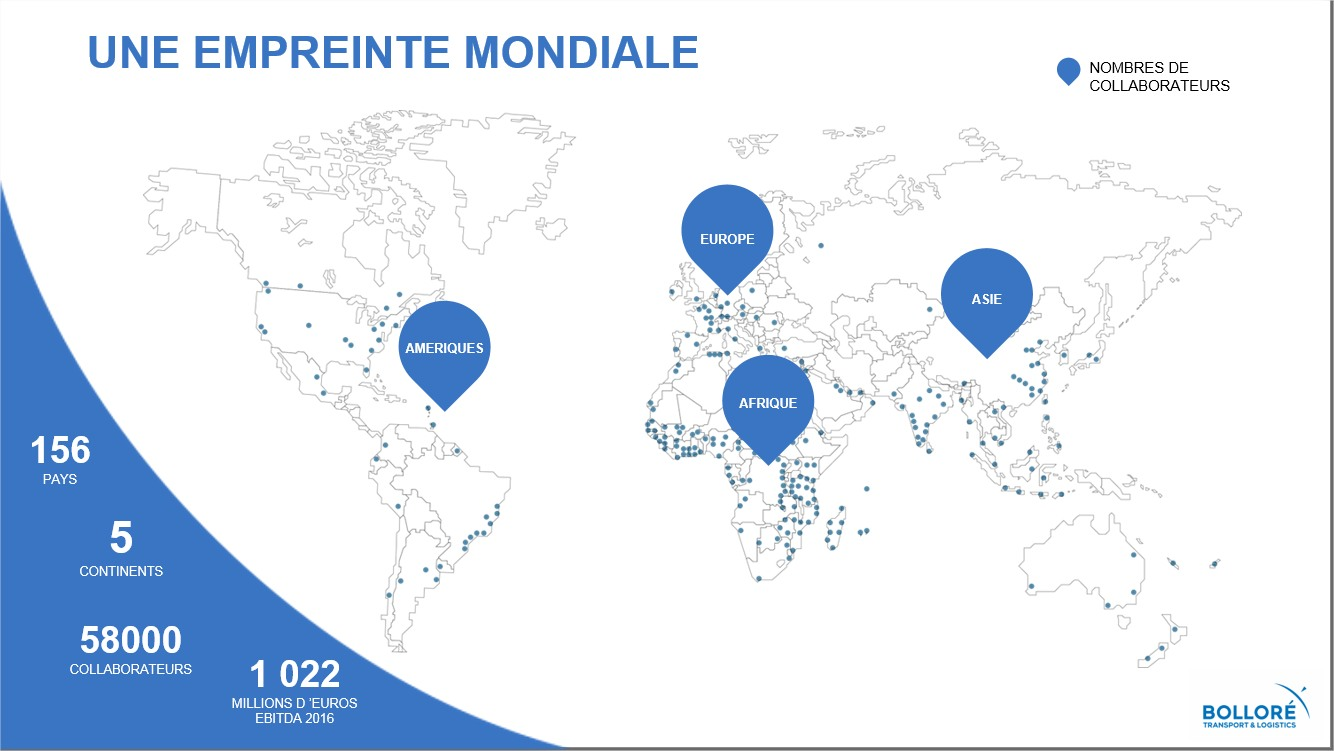
\includegraphics[width=0.9\linewidth]{images_BOLLORE/emprunte}
	\end{center}
	\caption{BOLLORÉ, une emprunte mondiale}
	\label{fig:1}	
\end{figure}

\subsection{Les 3 activités clés de groupe BOLLORÉ}
%\addcontentsline{toc}{subsection}{Les 3 activités clés de groupe BOLLORÉ}

	\begin{center}
		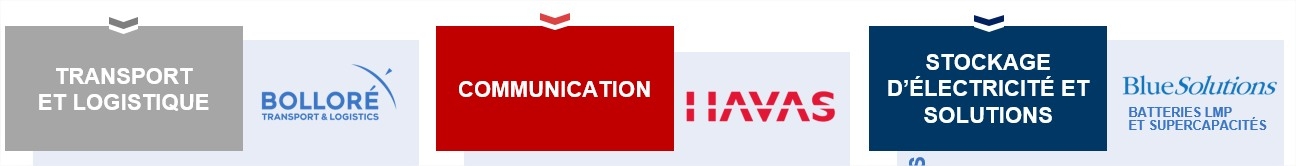
\includegraphics[width=1\linewidth]{images_BOLLORE/activite_bollore}
	\end{center}
	
\textcolor{black}{

\begin{itemize}
	\item	BOLLORÉ Transport & Logistique : 
\begin{itemize}
	\item Leader du transport et de la logistique en Afrique 
	\item Un des leaders mondiaux de la logistique et du freight forwarding
	\item Premier opérateur de concessions portuaires et ferroviaires en Afrique
	\item Acteur majeur de la logistique et de la distribution de produits pétroliers en France et en Europe. 
\end{itemize}

\item	HAVAS communication : 
\begin{itemize}
	\item Un des leaders mondiaux de la communication 
	\item Cnews Matin : second journal quotidien gratuit français 
	\item Bolloré Telecom, Wifirst : opérateur wifi et 4G	
\end{itemize}

\item	Stockage d’électricité et Solutions (Blue Solutions) : 
\begin{itemize}
	\item Applications Mobiles : Autopartage | Voiture électrique| Bus & Tram
	\item Applications stationnaires (Bluezone et Bluestorage): Buezone | Bluestorage
	\item Systèmes et services : IER | Polyconseil 
\end{itemize}
\end{itemize}
}

\subsection{BOLLORÉ TRANSPORT ET LOGISTICS}
%\addcontentsline{toc}{subsection}{BOLLORÉ TRANSPORT ET LOGISTICS}
\vspace{-0.5cm}
\begin{figure}[H]
	\begin{center}
		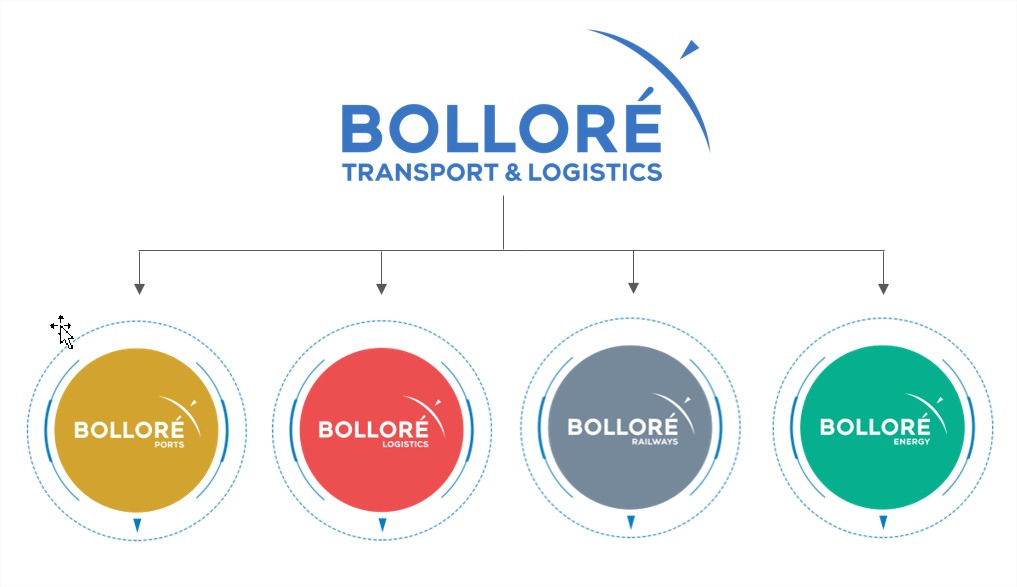
\includegraphics[width=0.55\linewidth]{images_BOLLORE/BTL}
	\end{center}
		\caption{Une marque, quatre métiers}
	\label{fig:2}	
\end{figure}

\begin{description}
	\item [BOLLORÉ PORTS] Opérateur leader en exploitations portuaires.
	\item [BOLLORÉ LOGISTICS] Acteur global du transport et de la logistique.
	\item [BOLLORÉ RAILWAYS]  Opérateur de trois concessions ferroviaires en Afrique.
	\item [BOLLORÉ ENERGY] Acteur majeur de la distribution et de la logistique pétrolière.
\end{description}

\subsection{Direction technique (DT) }
%\addcontentsline{toc}{subsection}{Direction technique (DT) }
\textcolor{black}{La Direction Technique se compose de 6 domaines (dont 3 transverses) assurant la conception, la mise en œuvre et le maintien en conditions opérationnelles des services qu’elle fournit.}
\begin{figure}[H]
	\begin{center}
			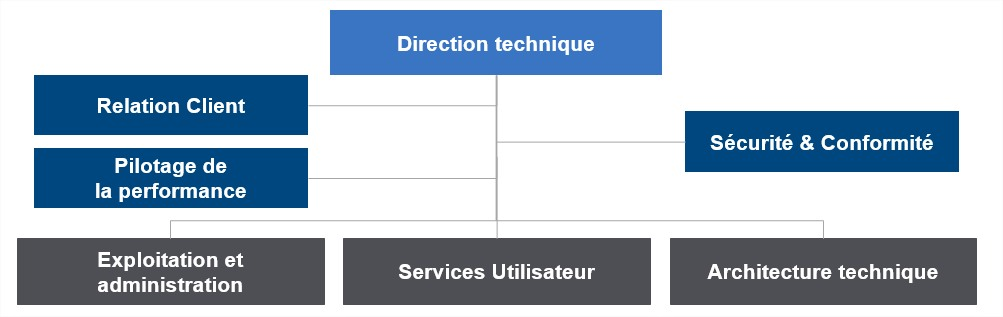
\includegraphics[width=1\linewidth]{images_BOLLORE/DT}
	\end{center}
	\caption{Organisation de la DT}
	\label{fig:3}	
\end{figure}

\section{Missions et perspectives }
%\addcontentsline{toc}{section}{Missions et perspectives }
\subsection{Projet Kaspersky Anti-Targetted Attack}
%\addcontentsline{toc}{subsection}{Projet Kaspersky Anti-Targetted Attack}
\textcolor{black}{Au sein de la cellule « Service de Sécurité Opérationnelle  » de la direction technique du groupe Bolloré Transports Logistics, le stagiaire aura comme missions :}
\begin{itemize}
	\item Assister la coordination de projets.
	\item Relation avec les éditeurs.
	\item Réalisera des documents de types : Cahiers de tests, Documents d’Architecture      Technique, Retours d’Expérience, Documents d’installation & de configuration, compte-rendu de réunions.
	\item Participera à des réunions.
\end{itemize}

\subsection{Migration OFFICE 365}
%\addcontentsline{toc}{subsection}{Migration OFFICE 365}
\textcolor{black}{Dans le cadre de la migration vers Office 365, le stagiaire aura comme missions :}
\begin{itemize}
	\item Consolider les données en une base de référence.
	\item Analyser les données.
	\item Réaliser des rapports visuels et des tableaux de bord via des outils décisionnels.
\end{itemize}
